\documentclass{article}
\usepackage[utf8]{inputenc}
\usepackage{multirow}
\usepackage{graphicx}

\begin{document}

\section{Introduction}
In this report I will explain a very crucial problem in our life, and how I addressed this problem using evolutionary computation in order to get to a satisfactory solution. The main idea is solving a maze while getting to the shortest path possible. I will explain the reasoning behind this problem and why a solution is necessary.
\section{Problem}
\subsection{Road and Traffic}
In our daily life, we use roads to get to places, sometimes important, such as jobs, interviews, schools, universities, etc. Many times of these, it is important to reach at a certain time, and we cannot really be late to some appointments.

\begin{figure}[htb!]
\centerline
{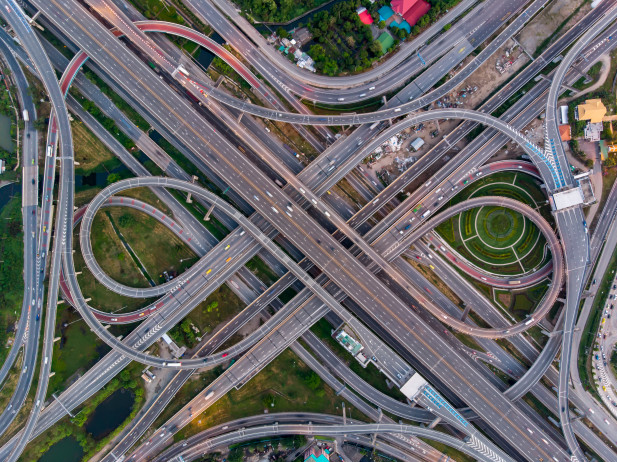
\includegraphics[width=130mm,scale=1.0]{roadtraffic.png}}
\caption{Road Traffic Looking Like a Maze}
\end{figure}

\subsection{Thought Process}
In order to design the problem in a way that can be solvable with evolutionary computation, I have looked at it as follows:
- Roads are made of directions and distances

- Distances can be converted to steps (units) in the final model

- Traffic either blocks a road or allows you to get around it by taking a longer path

- Program has to choose between bypassing the traffic in the same road by temporarily going into a different road or to find a completely different way

The final design was basically a maze, and the program has to go through it using evolutionary computation in order to find the path to the destination.

\subsection{Tokens}

I have achieved this using the following tokens:

- \# is basically a wall, or a unit you cannot go through

- . is an open area, you can freely move through it

- S is the starting point

- E is the ending point, or the destination

\begin{figure}[htb!]
\centerline
{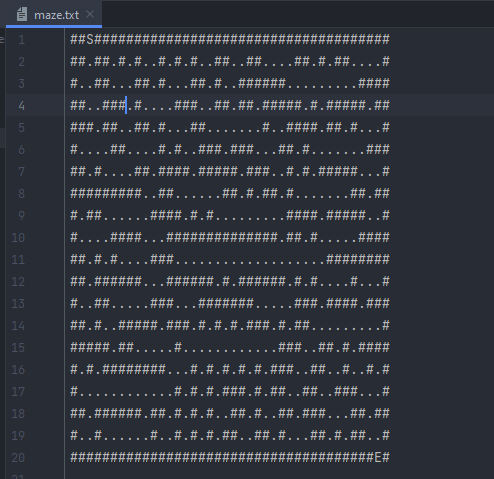
\includegraphics[width=65 mm,scale=1.0]{maze.png}}
\caption{Maze Example}
\end{figure}

\newpage

\section{Methodology}
As a result, I was able to design an implementation that would serve to act as a maze using Python. And then using genetic algorithm I was able to get to the destination. Every method used is explained by comments in it inside the code.

The program starts with an empty maze as you can see below:

\begin{figure}[htb!]
\centerline
{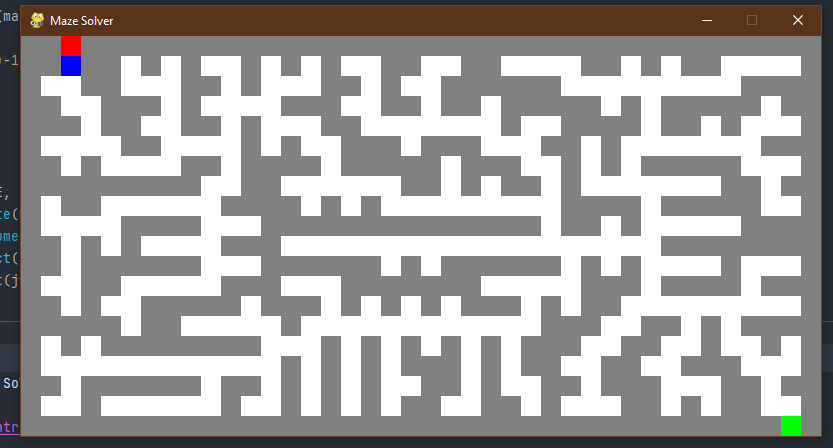
\includegraphics[width=130mm,scale=1.0]{emptmaze.png}}
\caption{Empty Maze}
\end{figure}

The text file is converted into a 2D map. White area is the dots in the text file, and it's the area that we are able to move through.

Gray area is the walls, or the area we are unable to go through.

Red is the starting block.

Green is the ending block.

Blue is the steps we have decided to take by using the steps taken by the best in each generation.

\newpage

As it is progressing, new generations are generated by going through different directions until a roadblock is hit, the best in each generation is selected each time and using it steps we can draw the directions taken on the map. This keeps going on repeat until the destination is reached.

\begin{figure}[htb!]
\centerline
{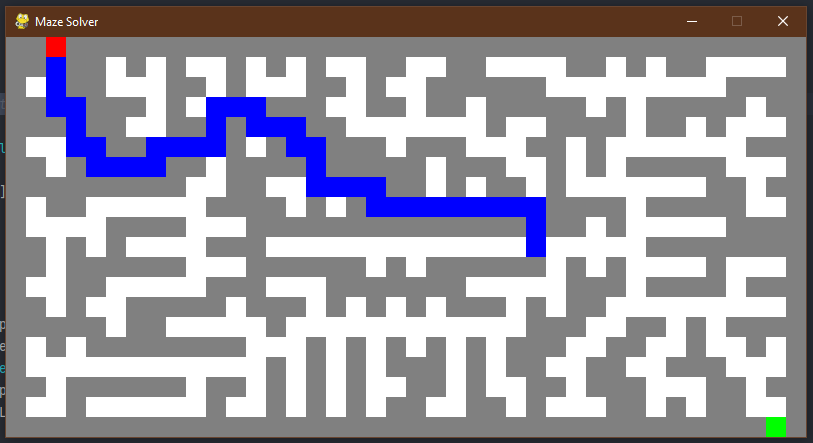
\includegraphics[width=130mm,scale=1.0]{mazeinprogress.png}}
\caption{Maze In Progress}
\end{figure}

While it's working, you can see the steps taken by the best in each generation in console, as well as the number of each generation.

\begin{figure}[htb!]
\centerline
{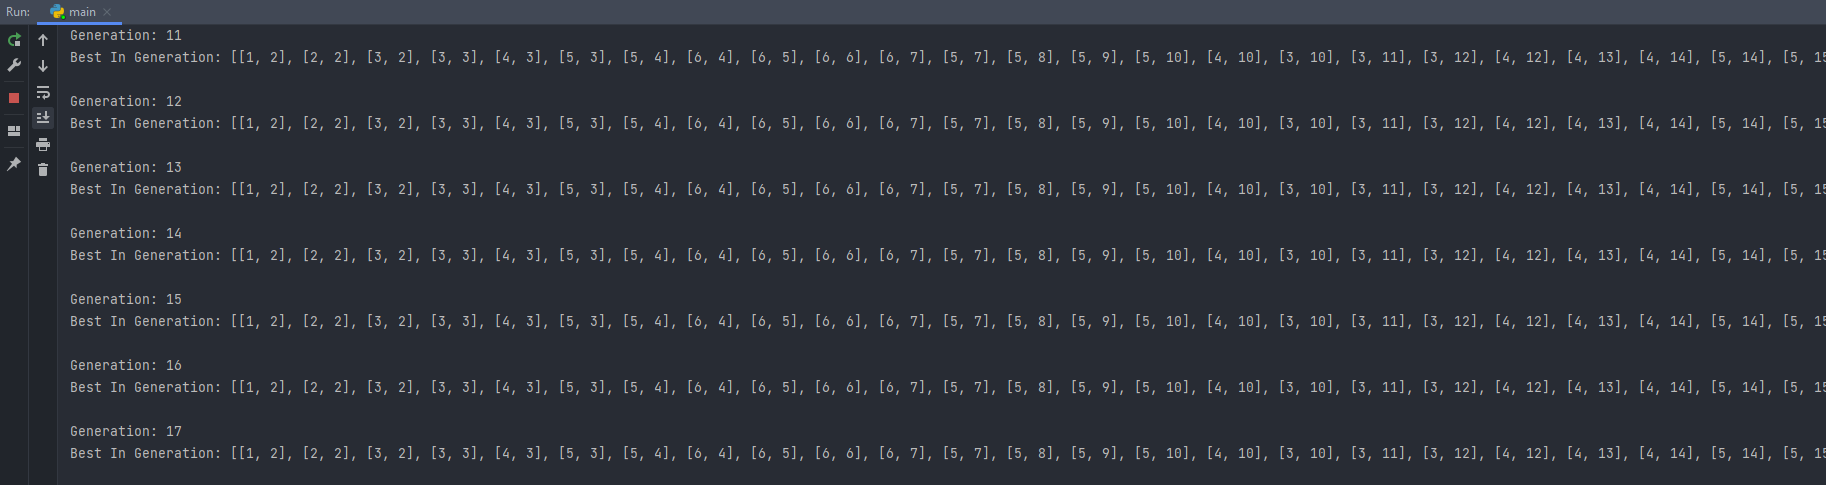
\includegraphics[width=130mm,scale=1.0]{generations.png}}
\caption{Generations}
\end{figure}
\newpage

\section{Results}
In the end, a final solution is reached, which gives us the steps we need to take to get through the maze. The final line in the console determines all the steps. It looks as follows

\begin{figure}[htb!]
\centerline
{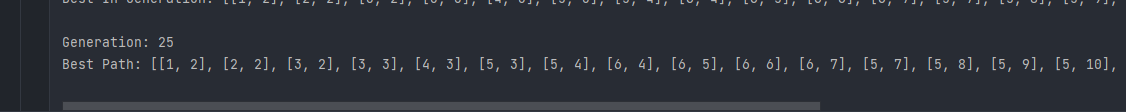
\includegraphics[width=130mm,scale=1.0]{finalsolution.png}}
\caption{Final Solution}
\end{figure}

The maze would finish drawing and the final result in the maze would look like this

\begin{figure}[htb!]
\centerline
{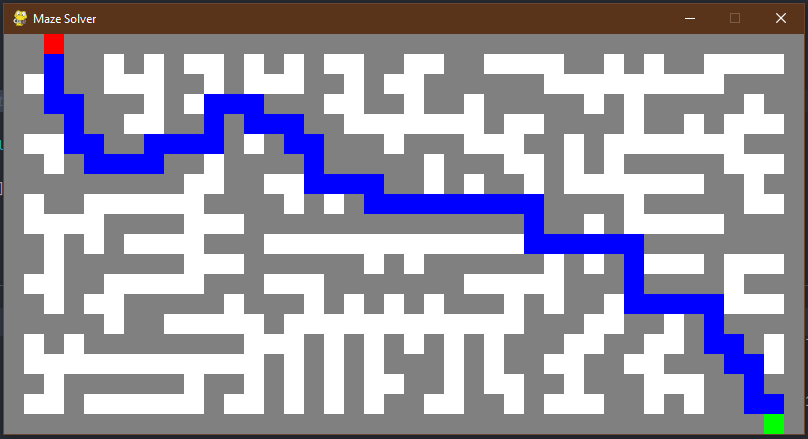
\includegraphics[width=130mm,scale=1.0]{mazefinal.png}}
\caption{Final Solution}
\end{figure}
\newpage


\section{Conclusion}
In conclusion, we have seen that:

- It is possible to draw a certain traffic point and roads between a starting and and ending destination

- We were able to make the solution solvable by providing a model that a program can read through and parse

- It was possible to utilize evolutionary computation through genetic algorithm to generate steps and get to a solution

- A final solution is made, and the steps required to take to get to the final solution are printed'

- The program realizes that the destination is reached and immediately stops upon reaching it
\\\\
And thus, the project is successful in that it was able to solve the maze and with that the road and traffic problem.


\end{document}
